\documentclass[conference]{IEEEtran}
\usepackage{blindtext, graphicx}
%\usepackage{cite}
% \cite{} output to follow that of IEEE. Loading the cite package will
% result in citation numbers being automatically sorted and properly
% "compressed/ranged". e.g., [1], [9], [2], [7], [5], [6] 
\usepackage[cmex10]{amsmath}

\usepackage[backend=biber]{biblatex}
\addbibresource{ref.bib}

% correct bad hyphenation here
%\hyphenation{op-tical net-works semi-conduc-tor}

\begin{document}
%
% paper title
% can use linebreaks \\ within to get better formatting as desired
\title{Predicting Readmission Rate of Diabetic Patients}


% author names and affiliations
% use a multiple column layout for up to three different
% affiliations
\author{\IEEEauthorblockN{Ashish Kumar}
\IEEEauthorblockA{Department of Mining Engineering\\
McGill University\\
ashish.kumar@mail.mcgill.ca}
\and
\IEEEauthorblockN{Charlie Bloomfield}
\IEEEauthorblockA{Department of Electrical and Computer Engineering\\
McGill University\\
charlie.bloomfield@mail.mcgill.ca}
\and
\IEEEauthorblockN{Jonathan Campbell}
\IEEEauthorblockA{School of Computer Science\\
McGill University\\
jonathan.campbell@mcgill.ca}}

% make the title area
\maketitle

%\boldmath

\begin{abstract}

Using an existing dataset of patient-hospital encounters, we present methodology for predicting the readmission of diabetic patients based on selected features of the encounters.

%This project gives an overview of the methods for predicting the readmission rates and classifying the diabetic patients based on their diagnoses, whether they are admitted before or after 30 days or not readmitted at all. An existing 10 years’ clinical database of 130 US hospitals was used for this project [1].

\end{abstract}

% An example of a floating figure using the graphicx package.
%\begin{figure}[!t]
%\centering
%\includegraphics[width=2.5in]{myfigure}
% where an .eps filename suffix will be assumed under latex, 
% and a .pdf suffix will be assumed for pdflatex; or what has been declared
% via \DeclareGraphicsExtensions.
%\caption{Simulation Results}
%\label{fig_sim}
%\end{figure}

% An example of a double column floating figure using two subfigures.
% (The subfig.sty package must be loaded for this to work.)
% The subfigure \label commands are set within each subfloat command, the
% \label for the overall figure must come after \caption.
% \hfil must be used as a separator to get equal spacing.
% The subfigure.sty package works much the same way, except \subfigure is
% used instead of \subfloat.
%
%\begin{figure*}[!t]
%\centerline{\subfloat[Case I]\includegraphics[width=2.5in]{subfigcase1}%
%\label{fig_first_case}}
%\hfil
%\subfloat[Case II]{\includegraphics[width=2.5in]{subfigcase2}%
%\label{fig_second_case}}}
%\caption{Simulation results}
%\label{fig_sim}
%\end{figure*}

% An example of a floating table. Note that, for IEEE style tables, the 
% \caption command should come BEFORE the table. Table text will default to
% \footnotesize as IEEE normally uses this smaller font for tables.
% The \label must come after \caption as always.
%
%\begin{table}[!t]
%% increase table row spacing, adjust to taste
%\renewcommand{\arraystretch}{1.3}
% if using array.sty, it might be a good idea to tweak the value of
% \extrarowheight as needed to properly center the text within the cells
%\caption{An Example of a Table}
%\label{table_example}
%\centering
%% Some packages, such as MDW tools, offer better commands for making tables
%% than the plain LaTeX2e tabular which is used here.
%\begin{tabular}{|c||c|}
%\hline
%One & Two\\
%\hline
%Three & Four\\
%\hline
%\end{tabular}
%\end{table}

\section{Introduction}

Diabetes affects 336 million people worldwide and is predicted to increase to 552 million in 2030 (missing ref)~\ref{missing}. Prediction of relevant factors resulting in readmission of diabetic patients is very important to reduce the large physical and finanical costs associated with readmission. This paper deals with the prediction of readmission of diabetic patients using a machine learning approach on a pre-existing dataset. We describe related research with said dataset in section 2, followed by a brief description of the dataset in section 3. Due to particularities with the dataset, several data pre-processing methods were performed and are discussed in section 4, followed by an explanation of the performance measurement criteria used in the project in section 5. We continue with brief descriptions of machine learning algorithms used, including baseline methods, with some focus on methods known to perform better on the dataset. The paper concludes with presentation and discussion of results.

\section{Related Work}

Diabetes or “diabetes mellitus” is a metabolic disorder characterized by hyperglycemia and disturbance of metabolism of fat protein and carbohydrates, caused by imperfections of insulin secretion or functioning~\cite{worldhealthorganization-2015}. Morbidity of patients in hospitals is significantly determined by the management of hyperglycemia in the hospitalized patients~\cite{hyperglycemia-2002, unrecognizeddiabetes-1998}. Readmission of patients to hospitals impacts the economy and quality of healthcare services. In terms of cost, readmission of patients cost the United States \$41.3 billion in 2011~\cite{missing}, out of which unchecked diabetes accounted for 23,700 readmissions at a cost of \$251 million~\cite{missing}. Rising readmission rates have prompted the Centers for Medicare \& Medicaid Services (CMS) to introduce measures to curb the problem~\cite{readmissionreduction-2015}.

The impact of HbA1c measurement on hospital readmission rates was studied with the same dataset we are using using a multivariate logistic regression algorithm~\cite{hba1c-2014}. Although the research showed the importance of this feature, a study of other relevant features was excluded. Another paper used a commercial Support Vector Machine algorithm (SAS Enterprise Miner) on the same dataset and obtained an accuracy of 63.7\%~\cite{missing (sas paper)}, but the handling of missing data was not properly managed and medical speciality of the attending doctor was removed, which is an important feature in deciding the outcome of the medical services rendered and eventually the readmission prediction. Furthermore, the measurement criteria used was the mis-classification rate, which is unreliable due to the imbalance of target classes. The demographics of diabetic patients were predicted using the same database in another paper on the same dataset~\cite{missing}, and the authors obtained an accuracy of 53.3\% using an ensemble method of decision trees.

\section{Dataset Description \& Analysis}

% discuss presence of missing data, what the features are, amount, where dataset came from...

A ten-year clinical database of 130 U.S. hospitals was used for our target prediction task~\cite{dataset-2014, hba1c-2014}. The dataset has 101,766 instances with 49 features (demographics, diagnoses, hbA1c measurement, etc.) with one target feature. The features are categorical and continuous and were encoded as described in the appendix for the application of machine learning algorithms. The number of possible value after encoding for each features is mentioned in Figure 1.

Duplicate encounters of patients were removed from the database to satisfy the I.I.D (Independent and Identically Distributed) assumption of the classification algorithms. Class imbalance and problems of missing data are described and dealt in Sections 4.2 and 4.3 respectively.

Figure 1. Description of database

\section{Data Pre-processing}

% discuss categorization of data
% smote, over sampling

\subsection{Feature Selection}

% removal of certain features not relevant (as per paper), possible combination of target into 2 classes...

\subsection{Data Imputation}

% deletion of missing data, using model-based approach to fill in values...

\section{Performance Measurement Criteria}

% f1 score, problems with that...

\section{Methodology}

\subsection{Baseline learners}

\subsection{Support Vector Machines}

\subsection{Adaboost}

\section{Results}

\begin{figure}[htpb]
	\centering
	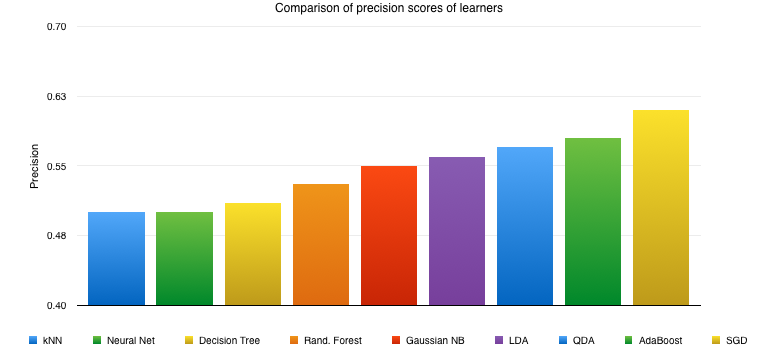
\includegraphics[width=0.5\textwidth]{learner_comparison}
	\caption{Comparison of precision scores of learners on dataset with missing data deleted and no oversampling performed.}
	\label{fig:learner_comp}
\end{figure}

Figure~\ref{fig:learner_comp} shows the precision scores of the various methods discussed above. Results across the board were not particularly impressive compared to the random baseline of 0.333, ranging from 0.49 to 0.61. k-Nearest Neigbor and Neural Net performed the worst. The highest-performing algorithm was the Support Vector Machine (SGD), followed by AdaBoost.

\begin{figure}[htpb]
	\centering
	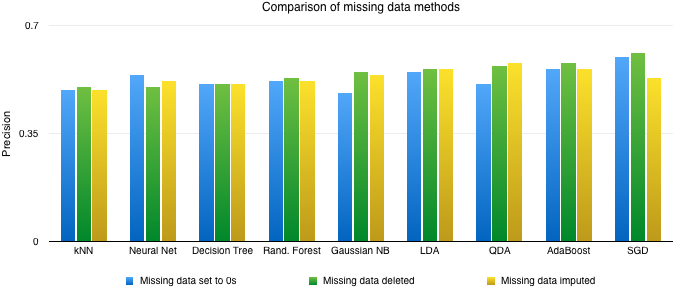
\includegraphics[width=0.5\textwidth]{missing_data_comparison}
	\caption{Comparison of missing data methods via precision scores of learners.}
	\label{fig:missing_data_comp}
\end{figure}

A comparison of the various methods to handle missing data is presented in figure~\ref{fig:missing_data_comp}, with precision scores from all learners shown. Generally, missing data set to its own category performed worse than both deletion and imputation, which each performed equally on average. There are some exceptions to this trend, specifically with Neural Networks, Gaussian Naive Bayes, and SVM, where one method is slightly better or worse than the other two.

\begin{figure}[htpb]
	\centering
	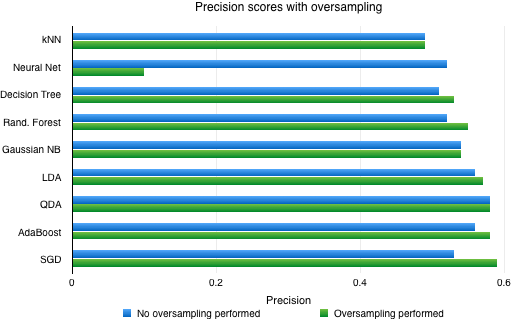
\includegraphics[width=0.5\textwidth]{oversampling_comparison}
	\caption{Precision scores of learners with and without oversampling of under-represented target classes, on a dataset with missing data deleted.}
	\label{fig:oversampling_comp}
\end{figure}

Figure~\ref{fig:oversampling_comp} shows the effect of oversampling on precision scores of the various learners. On average, oversampling of under-represented target classes performed equal to or better than not oversampling, particularly with SGD where the score improved by 0.6. One significant outlier was the Neural Network algorithm, where oversampling performed much worse than not oversampling.

\begin{figure}[htpb]
	\centering
	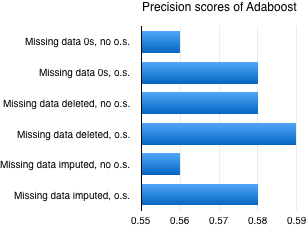
\includegraphics[width=0.5\textwidth]{adaboost}
	\caption{Precision scores of Adaboost learner for various data pre-processing combinations.}
	\label{fig:adaboost}
\end{figure}

The combinations of missing data methods and oversampling are presented in figure~\ref{fig:adaboost} with precision scores using the Adaboost algorithm. Results were very similar across the combinations, with scores only ranging from 0.56 to 0.59. Deleting missing data and oversampling performed the best at 0.59, while not performing oversampling and either imputing missing data or setting it to a separate category performed the worst at 0.56.

\begin{figure}[htpb]
	\centering
	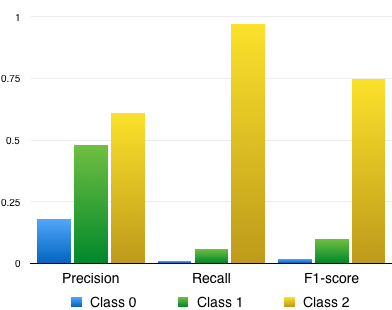
\includegraphics[width=0.5\textwidth]{full_results}
	\caption{Sample results of SGD learner on dataset with imputed missing data.}
	\label{fig:full_results}
\end{figure}

Precision, recall, and f1-score metrics for the three target classes using a sample learner (Support Vector Machines) with imputation for missing data is shown in figure~\ref{fig:full_results}. Although average values for each metric seem relatively stable (0.53 for precision, 0.60 for recall and 0.48 for f1-score), looking deeper at the breakdown of class values show an imbalance, with class 1 performing much worse than class 2, and class 2 performing much worse than class 3.

\begin{figure}[htpb]
	\centering
	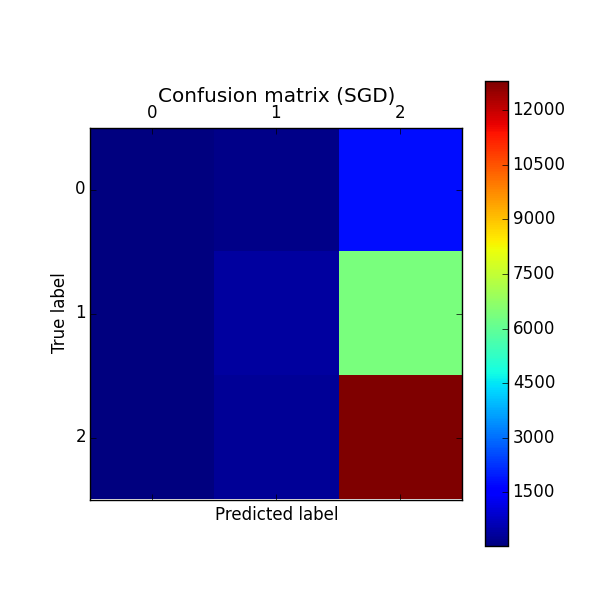
\includegraphics[width=0.5\textwidth]{full_results_confmatrix_SGD_md=imputed_ns=all_nc=3_os=f_test}
	\caption{Confusion matrix of SGD learner on dataset with imputed missing data.}
	\label{fig:full_results_cm}
\end{figure}

The confusion matrix for figure~\ref{fig:full_results} is shown in figure~\ref{fig:full_results_cm}. This figure displays that the majority of predictions are for class 2, even when the true class is 0 or 1. There are relatively much fewer predictions of class 0 or 1.

\section{Discussion}

\section{Conclusion}

\section{Future Work}


% if have a single appendix:
%\appendix[Proof of the Zonklar Equations]
% or
%\appendix  % for no appendix heading
% do not use \section anymore after \appendix, only \section*
% is possibly needed

% use appendices with more than one appendix
% then use \section to start each appendix
% you must declare a \section before using any
% \subsection or using \label (\appendices by itself
% starts a section numbered zero.)
%


\appendices
\section{Statement of Contributions}
Ashish - \par
Charlie - \par
Jonathan - \par

We hereby state that all work presented in this report is that of the authors.

% references section

% can use a bibliography generated by BibTeX as a .bbl file
% BibTeX documentation can be easily obtained at:
% http://www.ctan.org/tex-archive/biblio/bibtex/contrib/doc/
% The IEEEtran BibTeX style support page is at:
% http://www.michaelshell.org/tex/ieeetran/bibtex/
%\bibliographystyle{IEEEtran}
% argument is your BibTeX string definitions and bibliography database(s)
%\bibliography{IEEEabrv,../bib/paper}
%
% <OR> manually copy in the resultant .bbl file
% set second argument of \begin to the number of references
% (used to reserve space for the reference number labels box)
%\begin{thebibliography}{1}
%\end{thebibliography}

\printbibliography

% i still have to turn these refs into bibtex...
%[2]. Lakshminarayan, Kamakshi, et al. "Imputation of Missing Data Using Machine Learning Techniques." KDD. 1996.
%[3]. Batista, Gustavo EAPA, and Maria Carolina Monard. "An analysis of four missing data treatment methods for supervised learning." Applied Artificial Intelligence 17.5-6 (2003): 519-533.
%[4]. Lakshminarayan, Kamakshi, Steven A. Harp, and Tariq Samad. "Imputation of missing data in industrial databases." Applied Intelligence 11.3 (1999): 259-275.
%[5]. Purwar, Archana, and Sandeep Kumar Singh. "Issues in data mining: A comprehensive survey." Computational Intelligence and Computing Research (ICCIC), 2014 IEEE International Conference on. IEEE, 2014.
%[6]. N. Abe, “Sampling approaches to learning from imbalanced datasets: active learning, cost sensitive learning and beyond,” ICML-KDD'2003 Workshop: Learning from Imbalanced Data Sets, 2003.
%[7]. V. López, A. Farnandez, J.M. Torres, and F. Herrera et al,” Analysis of preprocessing vs. cost-sensitive learning for imbalanced classification. Open problems on intrinsic data characteristics”, Expert Systems with Applications, vol 39, pp. 6585–6608, 2012.
%[8]. G. Wu E. Y. Chang,”Class-Boundary Alignment for Imbalanced Dataset Learning,” ICML-KDD'2003 Workshop: Learning from Imbalanced Data Sets, 2003.
%[9]. B. Raskutti and A.Kowalcyzk, “Extreme Re-balancing for SVM's: a case study,” ICML-KDD'2003 Workshop: Learning from Imbalanced Data Sets, 2003.
%[10]. G. M. Weiss and F.Provost ,” Learning when training data are costly: The effect of class distribution on tree induction,” Journal of Artificial Intelligence Research, vol. 19, pp. 315–354. October 2003.
%[13]. http://www.who.int/diabetes/action_online/basics/en/
%[18] SAS paper

% biography section
% 
% If you have an EPS/PDF photo (graphicx package needed) extra braces are
% needed around the contents of the optional argument to biography to prevent
% the LaTeX parser from getting confused when it sees the complicated
% \includegraphics command within an optional argument. (You could create
% your own custom macro containing the \includegraphics command to make things
% simpler here.)
%\begin{biography}[{\includegraphics[width=1in,height=1.25in,clip,keepaspectratio]{mshell}}]{Michael Shell}
% or if you just want to reserve a space for a photo:

\begin{IEEEbiography}[{\includegraphics[width=1in,height=1.25in,clip,keepaspectratio]{picture}}]{John Doe}
\blindtext
\end{IEEEbiography}

% You can push biographies down or up by placing
% a \vfill before or after them. The appropriate
% use of \vfill depends on what kind of text is
% on the last page and whether or not the columns
% are being equalized.

%\vfill

% Can be used to pull up biographies so that the bottom of the last one
% is flush with the other column.
%\enlargethispage{-5in}


\end{document}